\documentclass[compress]{beamer}
\usepackage{ifthen,verbatim}

\newcommand{\isnote}{}
\xdefinecolor{lightyellow}{rgb}{1.,1.,0.25}
\xdefinecolor{darkblue}{rgb}{0.1,0.1,0.7}

%% Uncomment this to get annotations
%% \def\notes{\addtocounter{page}{-1}
%%            \renewcommand{\isnote}{*}
%% 	   \beamertemplateshadingbackground{lightyellow}{white}
%%            \begin{frame}
%%            \frametitle{Notes for the previous page (page \insertpagenumber)}
%%            \itemize}
%% \def\endnotes{\enditemize
%% 	      \end{frame}
%%               \beamertemplateshadingbackground{white}{white}
%%               \renewcommand{\isnote}{}}

%% Uncomment this to not get annotations
\def\notes{\comment}
\def\endnotes{\endcomment}

\setbeamertemplate{navigation symbols}{}
\setbeamertemplate{headline}{\mbox{ } \hfill
\begin{minipage}{5.5 cm}
\vspace{-0.75 cm} \small
\end{minipage} \hfill
\begin{minipage}{4.5 cm}
\vspace{-0.75 cm} \small
\begin{flushright}
\ifthenelse{\equal{\insertpagenumber}{1}}{}{Jim Pivarski \hspace{0.2 cm} \insertpagenumber\isnote/\pageref{numpages}}
\end{flushright}
\end{minipage}\mbox{\hspace{0.2 cm}}\includegraphics[height=1 cm]{../cmslogo} \hspace{0.1 cm} \includegraphics[height=1 cm]{../tamulogo} \hspace{0.01 cm} \vspace{-1.05 cm}}

\begin{document}
\begin{frame}
\vfill
\begin{center}
\textcolor{darkblue}{\Large Trigger Performance Review: Alignment}

\vfill
\begin{columns}
\column{0.3\linewidth}
\begin{center}
\large
\textcolor{darkblue}{Jim Pivarski}
\end{center}
\end{columns}

\begin{columns}
\column{0.3\linewidth}
\begin{center}
\scriptsize
{\it Texas A\&M University}
\end{center}
\end{columns}

\vfill
29 April, 2009

\end{center}
\end{frame}

%% \begin{notes}
%% \item This is the annotated version of my talk.
%% \item If you want the version that I am presenting, download the one
%% labeled ``slides'' on Indico (or just ignore these yellow pages).
%% \item The annotated version is provided for extra detail and a written
%% record of comments that I intend to make orally.
%% \item Yellow notes refer to the content on the {\it previous} page.
%% \item All other slides are identical for the two versions.
%% \end{notes}

\small

\begin{frame}
\frametitle{Alignment triggers}
\begin{itemize}
\item Large overlap with physics triggers: single/double muon, minbias
\begin{itemize}
\item turn-on curves are not important for alignment performance; only need a source of tracks
\item from Feb 4 Trigger Review: lean-menu physics triggers satisfy alignment needs
\end{itemize}

\item Specialized alignment triggers:
\begin{enumerate}
\item tracker-pointing cosmic rays: visible progress toward implementation
\item BSC beam-halo: see Gaelle's talk
\item CSC beam-halo: see Joe's talk
\end{enumerate}
\end{itemize}

\vfill
\hspace{-0.83 cm} \textcolor{darkblue}{\Large In this talk:}
\begin{itemize}
\item Status update on tracker-pointing cosmic ray trigger
\item Alignment performance and diagnostic with cosmic rays
\item Alignment performance with CSC beam-halo
\end{itemize}
\end{frame}

\begin{frame}
\frametitle{Tracker-pointing cosmics}

\begin{itemize}
\item Need to collect cosmic rays during collisions because
\begin{itemize}\setlength{\itemsep}{0.1 cm}
\item non-projective tracks constrain systematic distortions (!)
\item they offer ``live'' diagnostics, such as track splitting
\item CRAFT-like runs before and after collisions would have limited
  applicability: $\mathcal{O}(\mbox{100~$\mu$m})$ variations from
  time-dependent effects ($\vec{B}$, stress, temperature,
  humidity\ldots)
\end{itemize}
\end{itemize}

\hspace{-0.83 cm} \textcolor{darkblue}{\Large Status}

\begin{itemize}\setlength{\itemsep}{0.25 cm}
\item L1 emulator (Andr\'es Osorio)
\begin{itemize}\setlength{\itemsep}{0.1 cm}
\item mature in offline testing, code in CVS since January 2009
\item started integrating into CMSSW release with 3\_1\_0\_pre5
\end{itemize}

\item HLT\_TrackerCosmics (Yohann Tschudi)
\begin{itemize}\setlength{\itemsep}{0.1 cm}
\item still just a pointer to L1, but in the latest menu
\item studying tracker-pointing features of L1; no plots yet
\item developing reconstruction for cosmic rays mixed with minbias
\end{itemize}
\end{itemize}

\end{frame}

\begin{frame}
\frametitle{Alignment with cosmics}
\framesubtitle{From Andrei Gritsan's Trigger Review talk:}

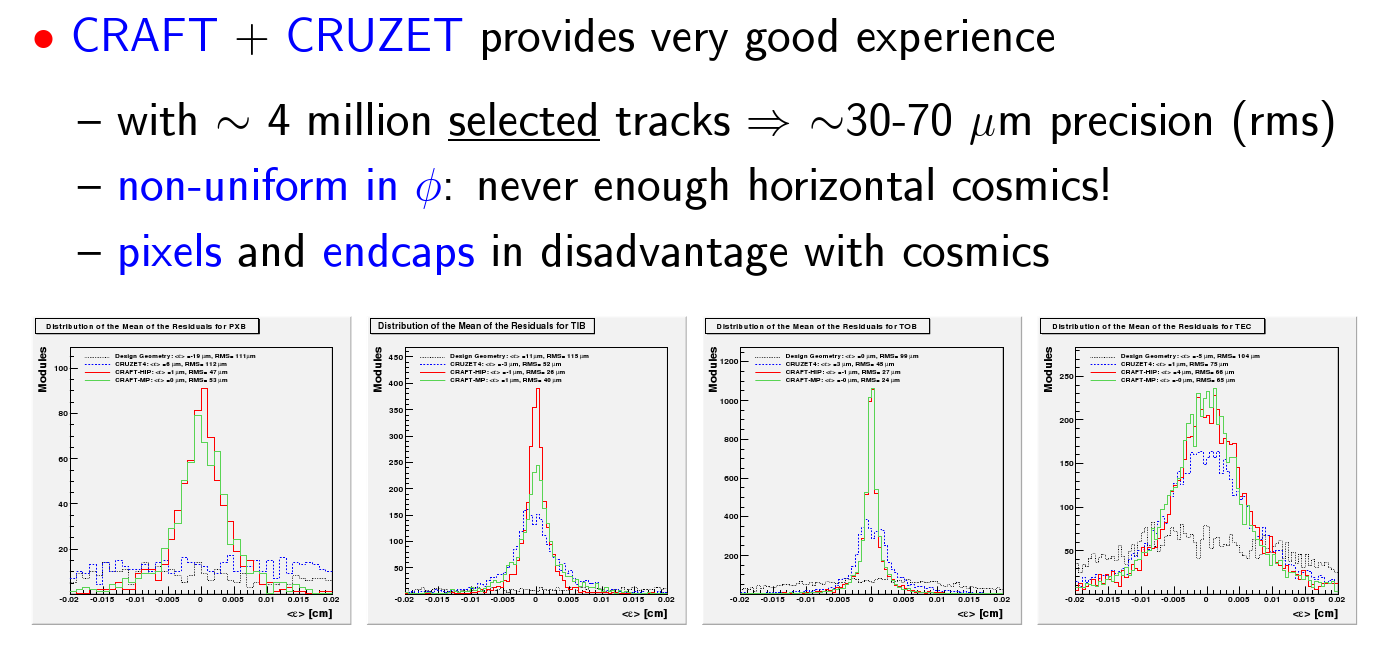
\includegraphics[width=0.85\linewidth]{andrei1.png}

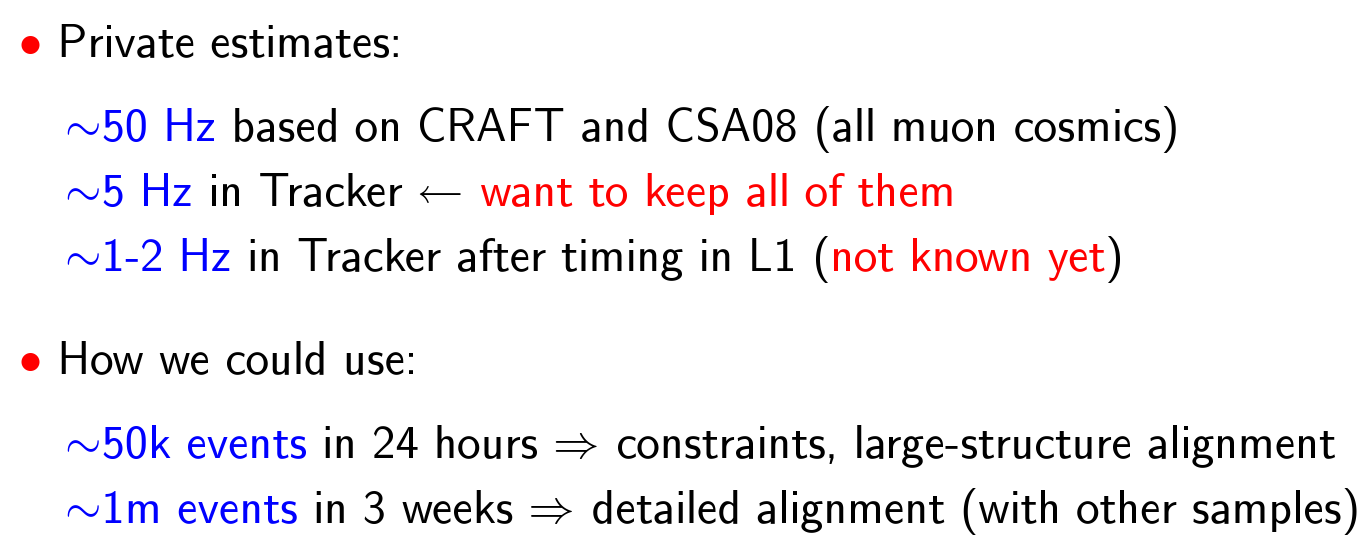
\includegraphics[width=0.85\linewidth]{andrei2.png}

\end{frame}

\begin{frame}
\frametitle{``Track splitting'' diagnostic}

\begin{columns}
\column{0.65\linewidth}
\begin{itemize}
\item Single cosmic ray muon is reconstructed as two LHC-like tracks
\item Mismatch in parameters at origin is purely instrumental
\item Only way to measure resolution of all 5 track parameters in data
\end{itemize}

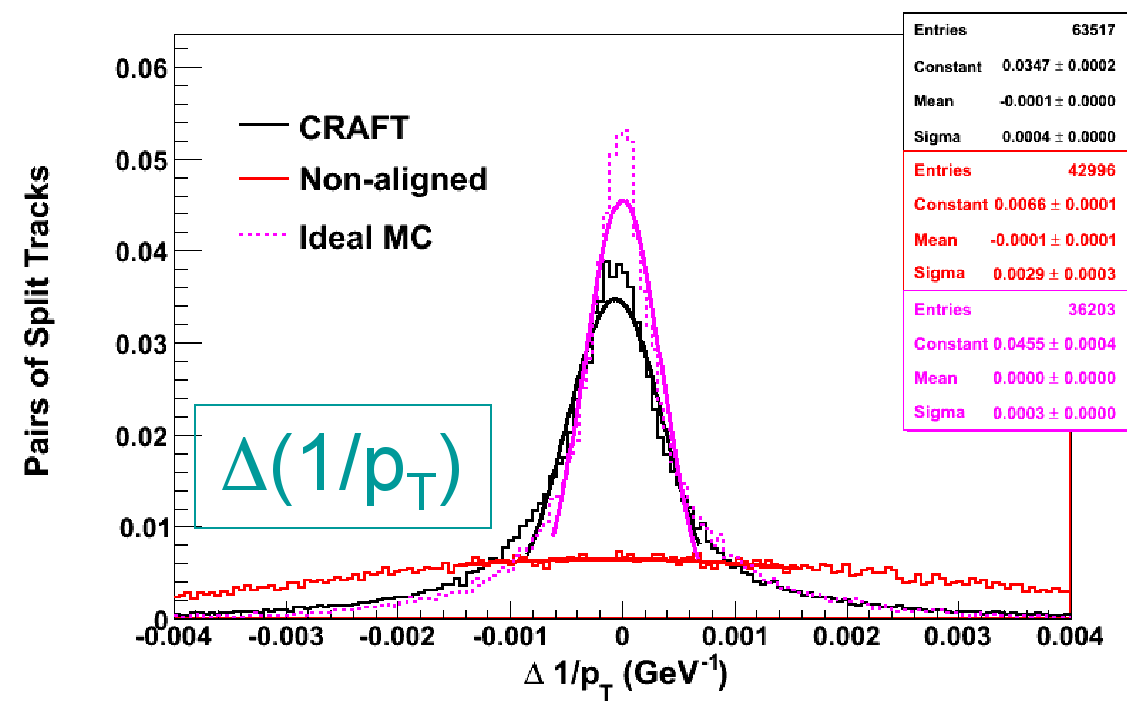
\includegraphics[width=\linewidth]{track_splitting.png}

\column{0.45\linewidth}
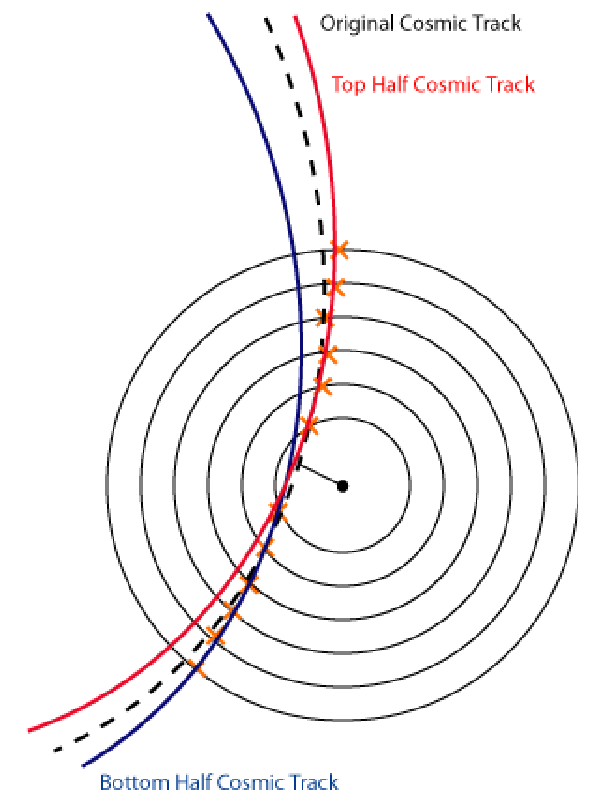
\includegraphics[width=\linewidth]{track_splitting_diagram.png}
\end{columns}

\hfill \scriptsize \textcolor{darkblue}{Alessio Bonato, Andrei Gritsan, Nhan Tran}
\end{frame}

\begin{frame}
\frametitle{Rate needed for diagnostics}

\begin{itemize}
\item 1\% precision in resolution measurement from 0.9~million
  SuperPointing cosmic rays in 15~million TrackerPointing dataset
\item $\sigma_\sigma = \mbox{1\%} \sqrt{\dfrac{15 \times 10^6}{\mbox{\textcolor{darkblue}{1--2 Hz}} \cdot t}}$, or 1--2 days for a 10\% measurement
\end{itemize}

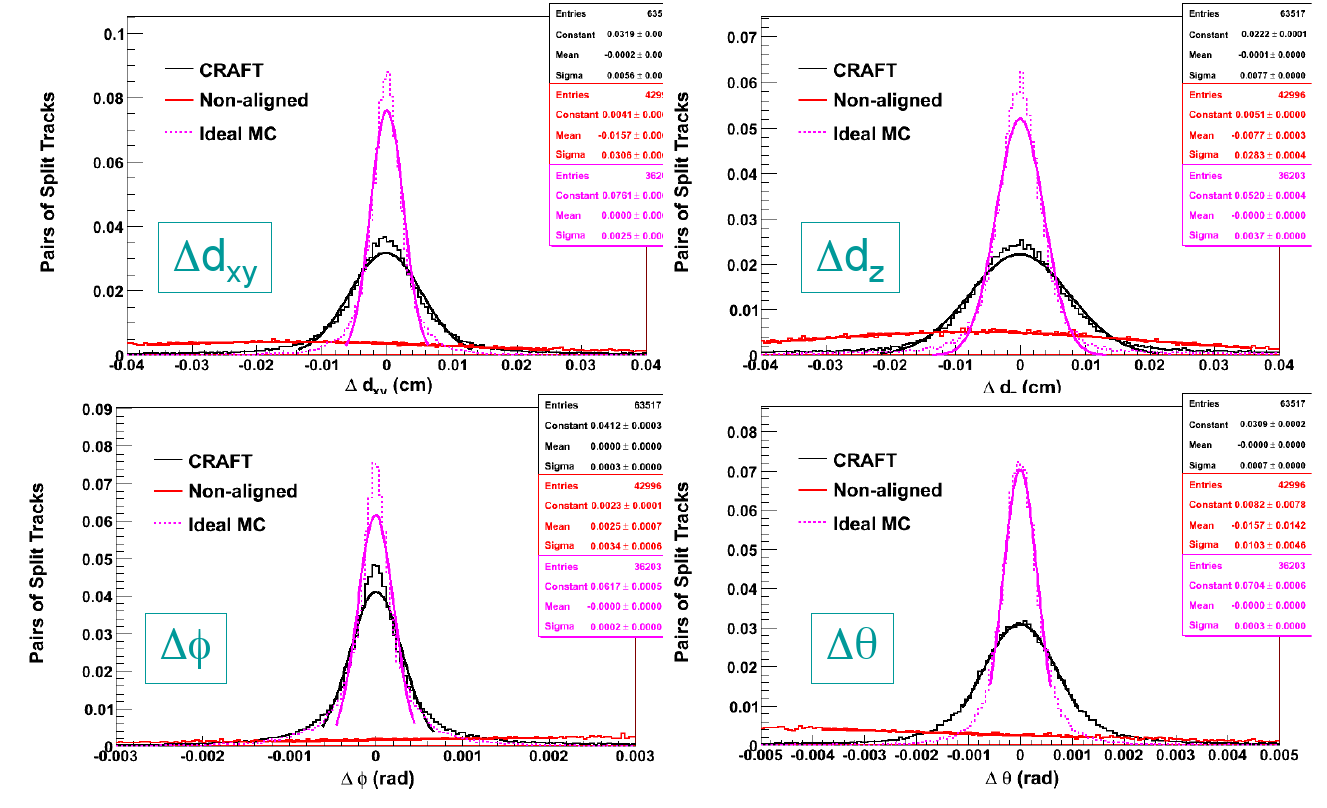
\includegraphics[width=0.9\linewidth]{track_splitting_other_parameters.png}
\end{frame}

\begin{frame}
\frametitle{\ldots for high-$p_T$ resolution}

\begin{itemize}
\item Only known way to measure $\mu$ resolution well above the $Z$ peak
\item Several hundred GeV: a qualitatively different environment
\begin{itemize}
\item $p_T$ of nearly straight tracks depends on muon spectrometer
\item muons create showers of delta rays in the tracking chambers
\end{itemize}
\item Cosmic ray spectrum drops as $E^{-2.7}$
\end{itemize}

\mbox{ } \hfill 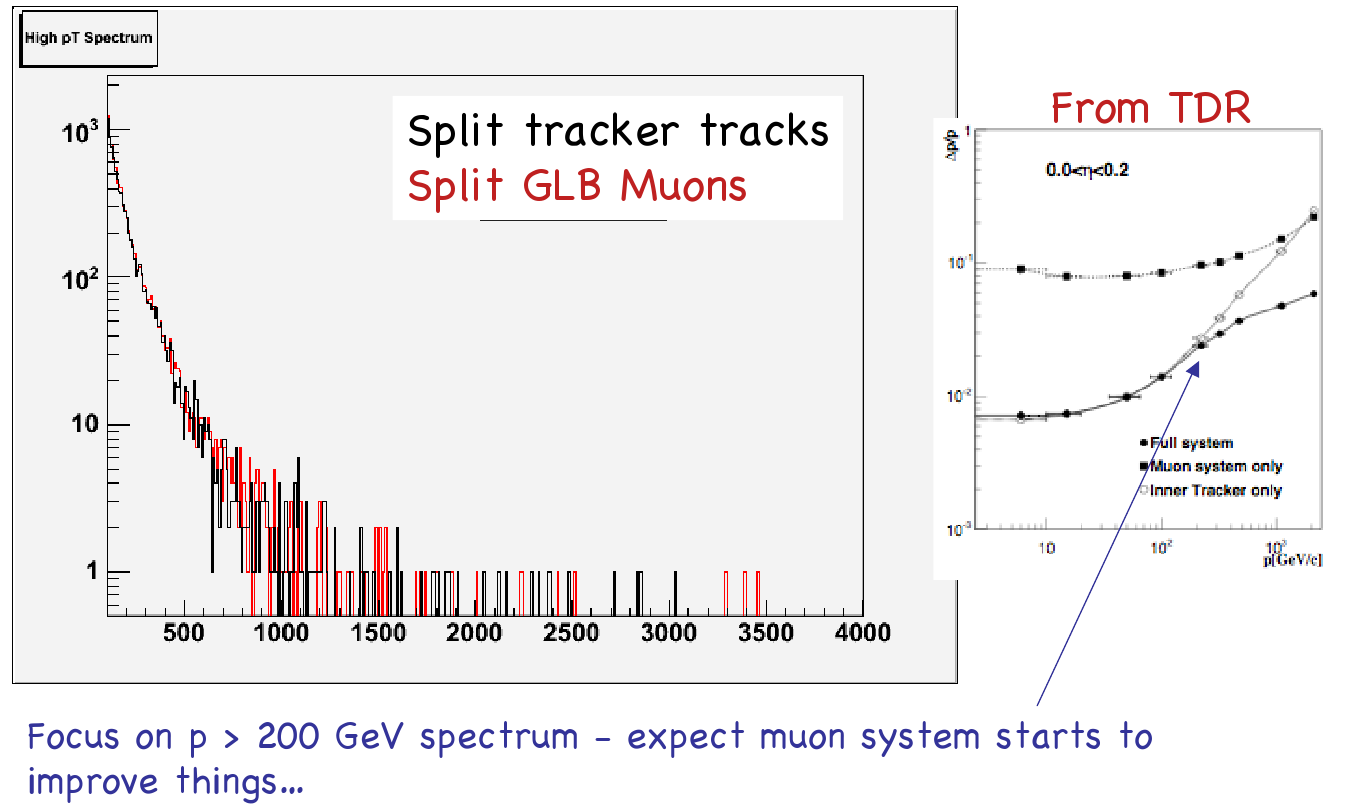
\includegraphics[width=0.85\linewidth]{track_splitting_high_pT.png} \hfill \mbox{ }
\end{frame}

\begin{frame}
\frametitle{Alignment with beam-halo}

\begin{columns}
\column{0.2\linewidth}
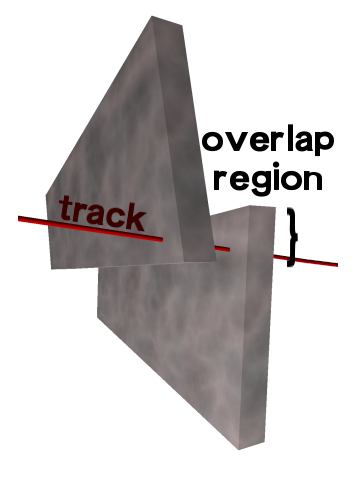
\includegraphics[width=\linewidth]{overlaps.png}

\column{0.8\linewidth}
\begin{itemize}
\item Beam-halo tracks passing through overlap of pairs of CSCs can be
  used to rapidly align with high precision

\item Demonstration with 9~minutes of 2008 LHC beam-halo: 270~$\mu$m
  accuracy verified by an independent method (photogrammetry)
\end{itemize}
\end{columns}

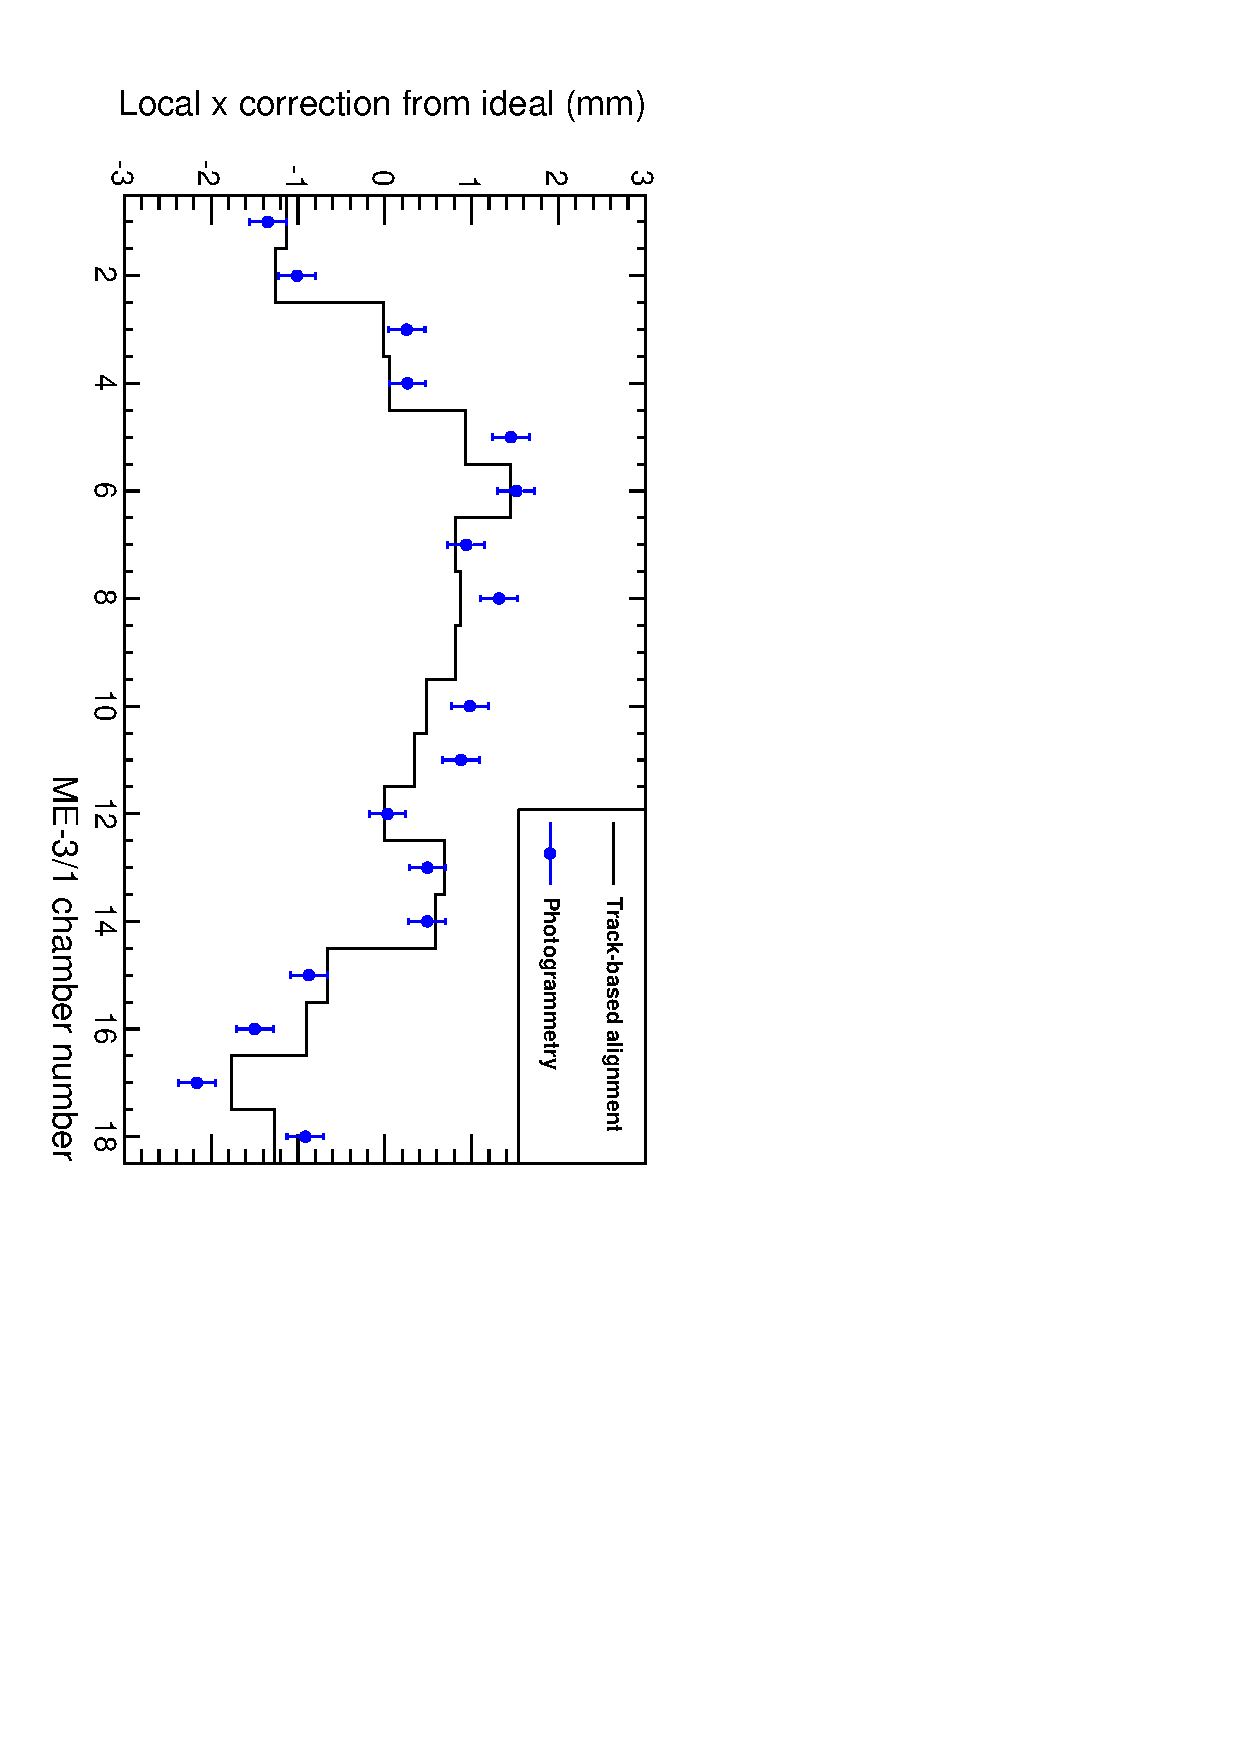
\includegraphics[width=3.8 cm, angle=90]{compare_m31_x.pdf} 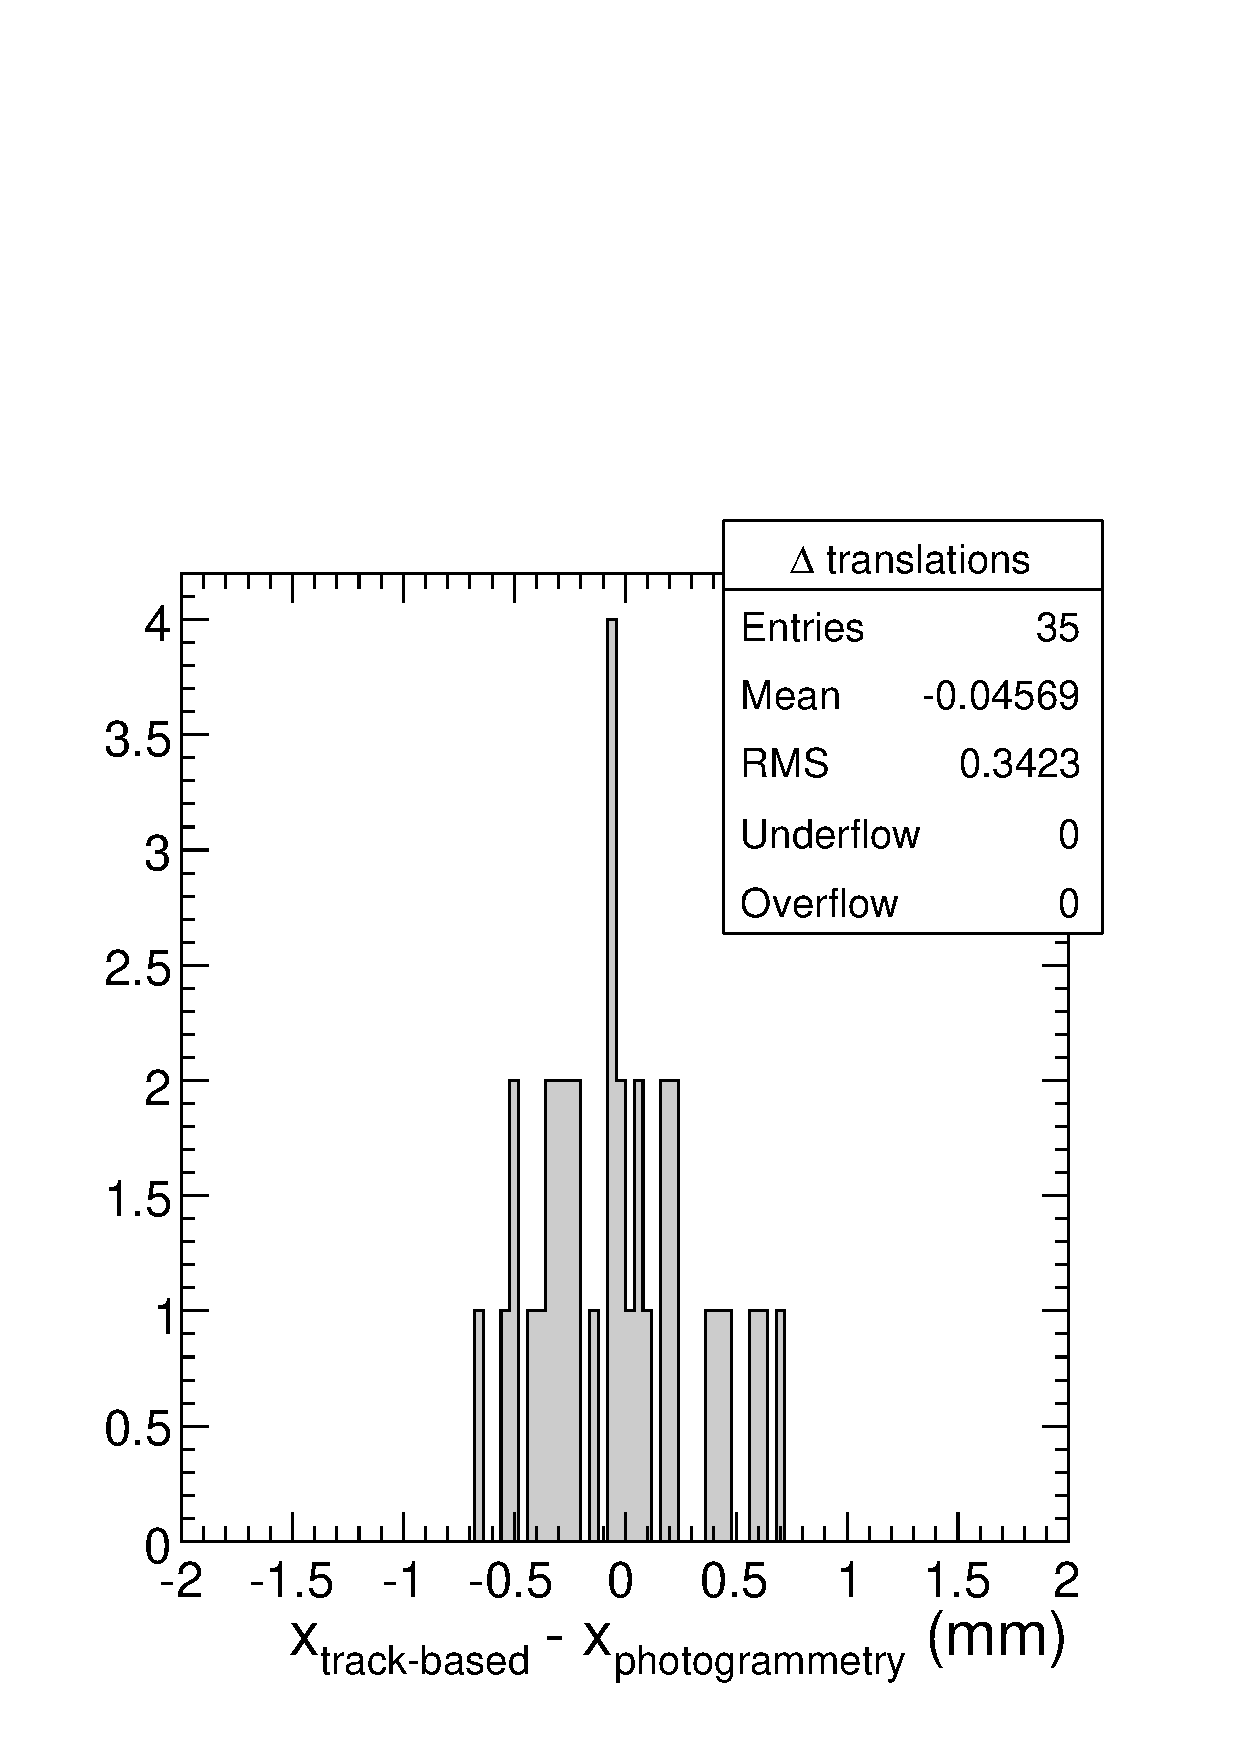
\includegraphics[height=3.8 cm]{delta_translations.pdf}

\begin{itemize}
\item Used 33,000 {\scriptsize HLT\_CSCBeamHaloOverlapsRing1} events for the above

\item For one alignment/day: {\scriptsize HLT\_CSCBeamHaloOverlapsRing1} at 0.4~Hz, \\
\textcolor{white}{For one alignment/day:} {\scriptsize HLT\_CSCBeamHaloOverlapsRing2} at 0.8~Hz
\end{itemize}
\end{frame}

\begin{frame}
\frametitle{Controlling beam-halo rate}

\begin{itemize}
\item Only tracks that pass through overlaps are strictly needed for alignment, about 5\% (from geometry; does not fluctuate)
\item Beam-halo rate is higher close to the beamline

\vspace{0.1 cm}
\mbox{\hspace{-1 cm} 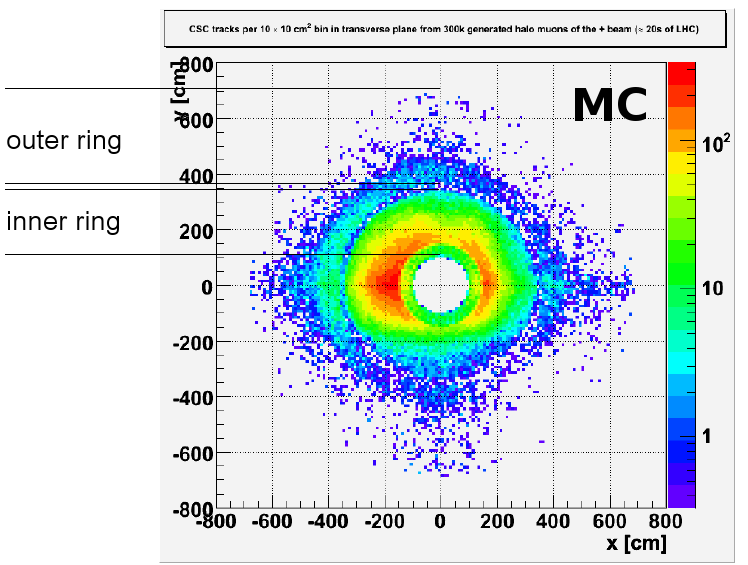
\includegraphics[height=0.33\linewidth]{beam-halo.png} 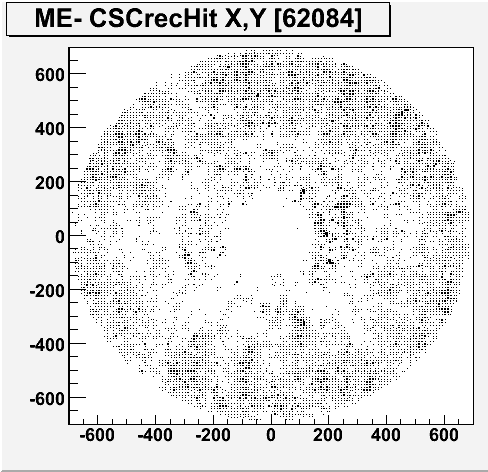
\includegraphics[height=0.33\linewidth]{spot_62084.png} 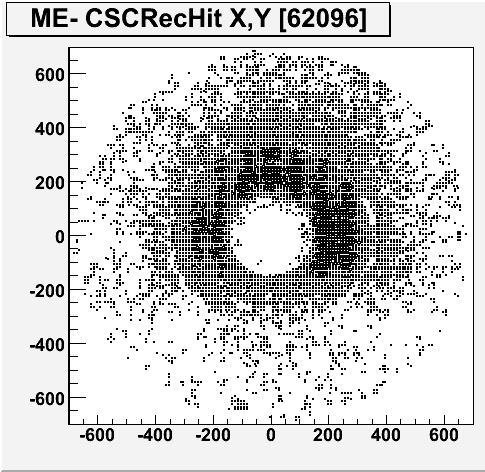
\includegraphics[height=0.33\linewidth]{spot_62096.png}}

\item Four HLT paths allow for tuning of prescales

\vfill
\begin{itemize}\setlength{\itemsep}{0.1 cm}
\item {\scriptsize HLT\_CSCBeamHalo} \hfill set by commissioning studies
\item {\scriptsize HLT\_CSCBeamHaloRing2or3} \hfill 2$\times$ (twice as many chambers)
\item {\scriptsize HLT\_CSCBeamHaloOverlapsRing1} \hfill 0.4~Hz
\item {\scriptsize HLT\_CSCBeamHaloOverlapsRing2} \hfill 0.8~Hz
\end{itemize}
\end{itemize}

\end{frame}

%% \section*{First section}
%% \begin{frame}
%% \begin{center}
%% \Huge \textcolor{blue}{First section}
%% \end{center}
%% \end{frame}

\begin{frame}
\frametitle{Conclusions}

\begin{itemize}\setlength{\itemsep}{0.25 cm}
\item Existing physics triggers are satisfactory for alignment needs
\item CRAFT and beam-halo experiences set estimates for alignment
  and diagnostic precision with specialized alignment triggers
\item Cosmic ray rate can't be increased above natural rate: 1--2~Hz
\begin{itemize}\setlength{\itemsep}{0.1 cm}
\item all of that will be needed for resolving global distortions
\item in-situ resolution diagnostics can be performed regularly
\item high-$p_T$ resolution will require longer accumulation of cosmics
\end{itemize}
\item Beam-halo rate can potentially be high and unpredictable
\begin{itemize}\setlength{\itemsep}{0.1 cm}
\item only 0.4$+$0.8~Hz needed to align the muon endcaps
\item trigger paths split by geometry to control fluctuations in rate
\end{itemize}
\item These are the same triggers that Gaelle and Joe will be \mbox{covering next\ldots\hspace{-1 cm}}
\end{itemize}

\label{numpages}
\end{frame}

\end{document}
